\documentclass{standalone}
\usepackage{tikz}
\usepackage{hsbcommon}



\begin{document}
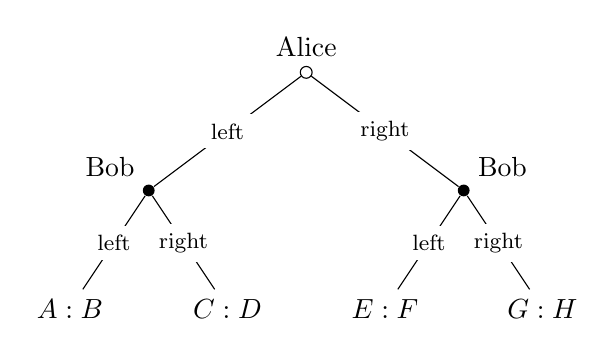
\begin{tikzpicture}[thin,
      level 1/.style={sibling distance=40mm},
      level 2/.style={sibling distance=20mm},
      level 3/.style={sibling distance=8mm},
      every circle node/.style={minimum size=1.5mm,inner sep=0mm}]
      
      \node[circle,draw,label=above:Alice] (root) {}
        child { node [circle,fill,label=above left:Bob] {}
          child { 
            node {$A:B$}
            edge from parent
              node[fill=white] {\footnotesize left}}
          child { 
            node {$C:D$}
            edge from parent
              node[fill=white] {\footnotesize right}}
          edge from parent
            node[fill=white] {\footnotesize left}}
        child { node [circle,fill,label=above right:Bob] {}
          child { 
            node {$E:F$}
              edge from parent
                node[fill=white] {\footnotesize left}}
          child { 
            node {$G:H$}
              edge from parent
                node[fill=white] {\footnotesize right}}
           edge from parent
             node[fill=white] {\footnotesize right}};

        % \node at (0,-4cm) {$T>R>S>P$};
    \end{tikzpicture}
\end{document}
